% !TeX program = xelatex
\documentclass[a4paper,oneside,openany]{extreport}
\usepackage{iftex}
\ifPDFTeX
  \errmessage{Báo cáo cần được biên dịch bằng XeLaTeX hoặc LuaLaTeX}
\fi

\usepackage{fontspec}
\IfFontExistsTF{Times New Roman}{%
  \setmainfont{Times New Roman}%
}{%
  \IfFontExistsTF{Tinos}{\setmainfont{Tinos}}{\setmainfont{TeX Gyre Termes}}%
}
\IfFontExistsTF{Times New Roman}{%
  \setsansfont{Times New Roman}
  \setmonofont{Times New Roman}
}{%
  \IfFontExistsTF{Tinos}{%
    \setsansfont{Tinos}
    \setmonofont{Tinos}
  }{%
    \setsansfont{TeX Gyre Termes}
    \setmonofont{TeX Gyre Termes}
  }%
}

\usepackage[vietnamese]{babel}
\usepackage[
  a4paper,
  top=3cm,
  bottom=3.5cm,
  left=3.5cm,
  right=2cm,
  headheight=15pt
]{geometry}

\usepackage{amsmath,amssymb}
\usepackage{graphicx}
\usepackage{pdfpages}
\usepackage{float}
\usepackage{placeins}
\usepackage{ragged2e}
\usepackage{indentfirst}
\usepackage{setspace}
\usepackage{titlesec}
\usepackage{tocloft}
\usepackage{etoolbox}
\usepackage{fancyhdr}
\usepackage{caption}
\usepackage{tabularx}
\usepackage{longtable}
\usepackage{array}
\usepackage{cellspace}
\usepackage{multirow}
\usepackage{enumitem}
\usepackage{xurl}
\usepackage{hyperref}
\usepackage{tikz}

\makeatletter
\renewcommand\normalsize{%
  \@setfontsize\normalsize{13pt}{15pt}%
  \abovedisplayskip 10pt plus 2pt minus 5pt%
  \abovedisplayshortskip \z@ plus 3pt%
  \belowdisplayshortskip 6pt plus 3pt minus 3pt%
  \belowdisplayskip \abovedisplayskip
  \let\@listi\@listI}
\renewcommand\small{\@setfontsize\small{12pt}{14pt}}
\renewcommand\footnotesize{\@setfontsize\footnotesize{10.5pt}{13pt}}
\renewcommand\large{\@setfontsize\large{14pt}{16pt}}
\renewcommand\Large{\@setfontsize\Large{16pt}{18pt}}
\renewcommand\LARGE{\@setfontsize\LARGE{18pt}{20pt}}
\makeatother

\AtBeginDocument{\normalsize\justifying\setlength{\parindent}{1cm}}
\frenchspacing
\setlength{\parindent}{1cm}
\setlength{\parskip}{0pt}
\setstretch{1.5}
\clubpenalty=10000
\widowpenalty=10000
\displaywidowpenalty=10000
\emergencystretch=2em

\renewcommand{\contentsname}{MỤC LỤC}
\renewcommand{\listfigurename}{DANH MỤC HÌNH}
\renewcommand{\listtablename}{DANH MỤC BẢNG}
\renewcommand{\bibname}{TÀI LIỆU THAM KHẢO}
\renewcommand{\figurename}{Hình}
\renewcommand{\tablename}{Bảng}
\addto\captionsvietnamese{%
  \renewcommand{\contentsname}{MỤC LỤC}%
  \renewcommand{\listfigurename}{DANH MỤC HÌNH}%
  \renewcommand{\listtablename}{DANH MỤC BẢNG}%
  \renewcommand{\bibname}{TÀI LIỆU THAM KHẢO}%
  \renewcommand{\figurename}{Hình}%
  \renewcommand{\tablename}{Bảng}%
}

\renewcommand{\thechapter}{\arabic{chapter}}
\renewcommand{\thesection}{\thechapter.\arabic{section}}
\renewcommand{\thesubsection}{\thesection.\arabic{subsection}}
\renewcommand{\thefigure}{\thechapter.\arabic{figure}}
\renewcommand{\thetable}{\thechapter.\arabic{table}}
\setcounter{secnumdepth}{2}
\setcounter{tocdepth}{2}

\titleformat{\chapter}[block]
  {\normalfont\bfseries\fontsize{14pt}{16pt}\selectfont\centering}
  {CHƯƠNG \thechapter.}
  {0.95cm}
  {}
\titlespacing*{\chapter}{0pt}{0pt}{8pt}

\titleformat{\section}[block]
  {\normalfont\bfseries\fontsize{13pt}{15pt}\selectfont}
  {\makebox[1cm][l]{\thesection.}}
  {0pt}
  {}
\titlespacing*{\section}{0.635cm}{8pt}{6pt}

\titleformat{\subsection}[block]
  {\normalfont\bfseries\fontsize{13pt}{15pt}\selectfont}
  {\makebox[1.35cm][l]{\thesubsection.}}
  {0pt}
  {}
\titlespacing*{\subsection}{1.27cm}{6pt}{5pt}

\captionsetup{
  font=normalsize,
  labelfont=normalfont,
  labelsep=colon,
  justification=centering,
  singlelinecheck=true
}
\captionsetup[figure]{position=bottom,skip=8pt}
\captionsetup[table]{position=top,skip=8pt}

\fancypagestyle{reportplain}{%
  \fancyhf{}
  \renewcommand{\headrulewidth}{0pt}
  \renewcommand{\footrulewidth}{0pt}
  \fancyfoot[C]{\thepage}
}
\fancypagestyle{plain}{%
  \fancyhf{}
  \renewcommand{\headrulewidth}{0pt}
  \renewcommand{\footrulewidth}{0pt}
  \fancyfoot[C]{\thepage}
}

\newlength{\UITFrontTitleAfterSkip}
\setlength{\UITFrontTitleAfterSkip}{12pt}

\renewcommand{\cftdotsep}{0.5}
\renewcommand{\cftchapfont}{\normalfont\normalsize}
\renewcommand{\cftchappagefont}{\normalfont\normalsize}
\renewcommand{\cftsecfont}{\normalfont\normalsize}
\renewcommand{\cftsecpagefont}{\normalfont\normalsize}
\renewcommand{\cftsubsecfont}{\normalfont\normalsize}
\renewcommand{\cftsubsecpagefont}{\normalfont\normalsize}
\setlength{\cftbeforechapskip}{3pt}
\setlength{\cftbeforesecskip}{0pt}
\setlength{\cftbeforesubsecskip}{0pt}
\setlength{\cftbeforefigskip}{0pt}
\setlength{\cftbeforetabskip}{0pt}

\makeatletter
\patchcmd{\@chapter}{\addtocontents{lof}{\protect\addvspace{10\p@}}}{}{}{}
\patchcmd{\@chapter}{\addtocontents{lot}{\protect\addvspace{10\p@}}}{}{}{}

\newcommand{\uitfronttitle}[1]{%
  \par\noindent\makebox[\textwidth][c]{%
    \bfseries\fontsize{14pt}{16pt}\selectfont #1%
  }%
  \par\vspace{\UITFrontTitleAfterSkip}%
}
\newcommand{\uitTOCSetup}{%
  \parindent=0pt\relax
  \parskip=0pt\relax
  \setstretch{1.5}%
  \let\addvspace\@gobble
  \let\babel@toc\@gobbletwo
}
\newcommand{\uittableofcontents}{%
  \clearpage
  \pagestyle{empty}%
  \thispagestyle{empty}%
  \begingroup
    \uitTOCSetup
    \uitfronttitle{MỤC LỤC}%
    \@starttoc{toc}%
    \thispagestyle{empty}%
  \endgroup
}
\newcommand{\uitlistoffigures}{%
  \clearpage
  \pagestyle{empty}%
  \thispagestyle{empty}%
  \begingroup
    \uitTOCSetup
    \uitfronttitle{DANH MỤC HÌNH}%
    \@starttoc{lof}%
    \thispagestyle{empty}%
  \endgroup
}
\newcommand{\uitlistoftables}{%
  \clearpage
  \pagestyle{empty}%
  \thispagestyle{empty}%
  \begingroup
    \uitTOCSetup
    \uitfronttitle{DANH MỤC BẢNG}%
    \@starttoc{lot}%
    \thispagestyle{empty}%
  \endgroup
}
\renewcommand{\tableofcontents}{\uittableofcontents}
\renewcommand{\listoffigures}{\uitlistoffigures}
\renewcommand{\listoftables}{\uitlistoftables}

\newcommand{\uitTOCDotLeaders}{\nobreak\leaders\hbox{\normalfont.\kern0.25pt}\hfill\nobreak}
\newcommand{\uitTOCPage}[1]{\makebox[1.2em][r]{#1}}
\renewcommand*{\l@chapter}[2]{%
  \begingroup
    \parindent=0pt\relax
    \normalfont\fontsize{12pt}{14pt}\selectfont
    \par\noindent
    \renewcommand*{\numberline}[1]{\makebox[2.75cm][l]{CHƯƠNG~##1.}\hspace{0.20cm}}%
    #1\uitTOCDotLeaders\uitTOCPage{#2}\par
  \endgroup
}
\renewcommand*{\l@section}[2]{%
  \begingroup
    \parindent=0pt\relax
    \normalfont\fontsize{12pt}{14pt}\selectfont
    \par\noindent\hspace*{0.5cm}%
    \renewcommand*{\numberline}[1]{\makebox[1.15cm][l]{##1.}}%
    #1\uitTOCDotLeaders\uitTOCPage{#2}\par
  \endgroup
}
\renewcommand*{\l@subsection}[2]{%
  \begingroup
    \parindent=0pt\relax
    \normalfont\normalsize
    \par\noindent\hspace*{1cm}%
    \renewcommand*{\numberline}[1]{\makebox[1.55cm][l]{##1.}}%
    #1\uitTOCDotLeaders\uitTOCPage{#2}\par
  \endgroup
}
\renewcommand*{\l@figure}[2]{%
  \begingroup
    \parindent=0pt\relax
    \normalfont\fontsize{12pt}{14pt}\selectfont
    \par\noindent
    \renewcommand*{\numberline}[1]{\makebox[2.05cm][l]{Hình~##1:}}%
    #1\uitTOCDotLeaders\uitTOCPage{#2}\par
  \endgroup
}
\renewcommand*{\l@table}[2]{%
  \begingroup
    \parindent=0pt\relax
    \normalfont\fontsize{12pt}{14pt}\selectfont
    \par\noindent
    \renewcommand*{\numberline}[1]{\makebox[2.05cm][l]{Bảng~##1:}}%
    #1\uitTOCDotLeaders\uitTOCPage{#2}\par\vspace{1.5pt}%
  \endgroup
}

\newlength{\UITBibItemSep}
\setlength{\UITBibItemSep}{5pt}
\renewenvironment{thebibliography}[1]{%
  \clearpage
  \phantomsection
  \addcontentsline{toc}{chapter}{TÀI LIỆU THAM KHẢO}%
  \begingroup
  \uitfronttitle{\bibname}%
  \RaggedRight
  \setlength{\parindent}{0pt}%
  \setstretch{1.5}%
  \list{\@biblabel{\@arabic\c@enumiv}}{%
    \settowidth\labelwidth{\@biblabel{#1}}%
    \setlength{\labelsep}{0.25cm}%
    \setlength{\leftmargin}{0.95cm}%
    \setlength{\itemsep}{\UITBibItemSep}%
    \setlength{\parsep}{0pt}%
    \setlength{\topsep}{0pt}%
    \usecounter{enumiv}%
    \let\p@enumiv\@empty
    \renewcommand\theenumiv{\@arabic\c@enumiv}%
  }%
  \sloppy\clubpenalty4000\widowpenalty4000
}{%
  \endlist
  \endgroup
}
\makeatother

\hypersetup{
  colorlinks=true,
  linkcolor=black,
  citecolor=black,
  urlcolor=black,
  pdfauthor={Lê Nguyễn Thành Danh; Trần Minh Nhật},
  pdftitle={Thiết kế IP xử lý và cảnh báo bụi mịn PM2.5 trên FPGA}
}
\urlstyle{same}

\setlist[itemize]{leftmargin=1.27cm,itemsep=0pt,topsep=4pt}
\setlist[enumerate]{leftmargin=1.27cm,itemsep=0pt,topsep=4pt}

\newcommand{\reporttablestretch}{1.00}
\newcommand{\reporttablecelllinespread}{1.50}
\newlength{\reporttablelinegap}
\setlength{\reporttablelinegap}{9.5pt}
\setlength{\cellspacetoplimit}{0.65\reporttablelinegap}
\setlength{\cellspacebottomlimit}{\reporttablelinegap}
\addparagraphcolumntypes{X}
\newcolumntype{L}[1]{>{\raggedright\arraybackslash}S{p{#1}}}
\newcolumntype{C}[1]{>{\centering\arraybackslash}S{p{#1}}}
\newcolumntype{Y}{>{\raggedright\arraybackslash}S{X}}
\newcolumntype{Z}{>{\centering\arraybackslash}S{X}}
\newcommand{\tableheader}[1]{\textbf{#1}}
\renewcommand{\arraystretch}{\reporttablestretch}
\setlength{\extrarowheight}{0pt}
\setlength{\arrayrulewidth}{0.5pt}
\setlength{\tabcolsep}{5pt}
\AtBeginEnvironment{tabular}{\setstretch{\reporttablecelllinespread}}
\AtBeginEnvironment{tabularx}{\setstretch{\reporttablecelllinespread}}
\AtBeginEnvironment{longtable}{\setstretch{\reporttablecelllinespread}}

\newcommand{\code}[1]{\texttt{#1}}
\newcommand{\pmunit}{\ensuremath{\mu\mathrm{g}/\mathrm{m}^{3}}}
\newcommand{\reportfigure}[4][0.88\linewidth]{%
  \begin{figure}[H]
    \centering
    \includegraphics[width=#1]{#2}
    \caption{#3}
    \label{#4}
  \end{figure}
}

\begin{document}
\hypersetup{pageanchor=false}
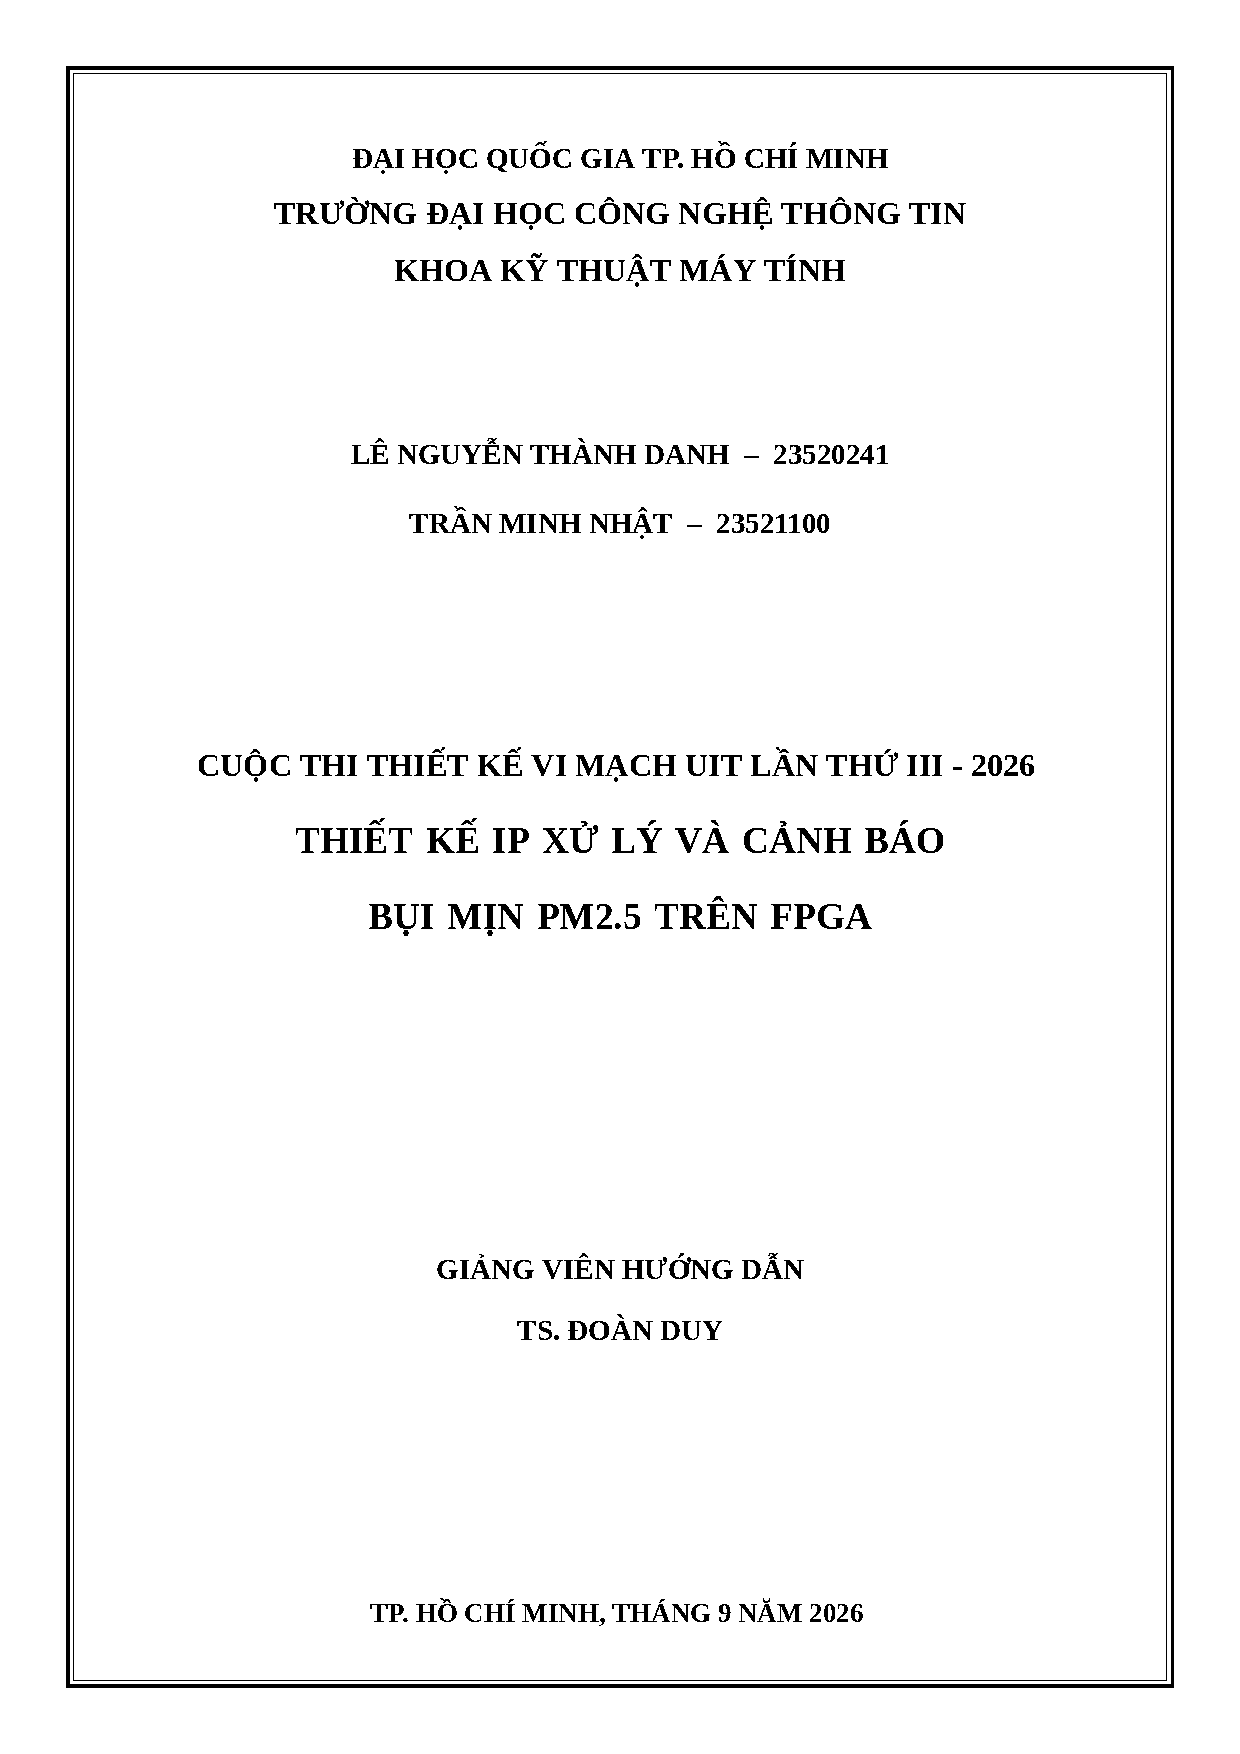
\includepdf[
  pages=1,
  fitpaper=true,
  pagecommand={\thispagestyle{empty}}
]{assets/official_cover.pdf}

\pagenumbering{gobble}
\pagestyle{empty}
\uittableofcontents
\uitlistoffigures
\uitlistoftables

\clearpage
\uitfronttitle{DANH MỤC TỪ VIẾT TẮT}
\begingroup
\fontsize{12pt}{14pt}\selectfont
\setlength{\tabcolsep}{5.5pt}
\setlength{\LTleft}{0pt plus 1fil}
\setlength{\LTright}{0pt plus 1fil}
\begin{longtable}{|C{0.14\textwidth}|C{0.33\textwidth}|C{0.41\textwidth}|}
\hline
\tableheader{Viết tắt} & \tableheader{Viết đầy đủ} & \tableheader{Ý nghĩa} \\
\hline
\endfirsthead
\hline
\tableheader{Viết tắt} & \tableheader{Viết đầy đủ} & \tableheader{Ý nghĩa} \\
\hline
\endhead
APB & Advanced Peripheral Bus & Bus ngoại vi dùng để truy cập thanh ghi của các khối ngoại vi trong SoC. \\
\hline
CAMS & Copernicus Atmosphere Monitoring Service & Dịch vụ quan trắc khí quyển Copernicus. \\
\hline
FPGA & Field-Programmable Gate Array & Mạch tích hợp có thể cấu hình lại tại hiện trường. \\
\hline
IP & Intellectual Property & Khối thiết kế phần cứng có thể tích hợp và tái sử dụng. \\
\hline
MAE & Mean Absolute Error & Sai số tuyệt đối trung bình. \\
\hline
PM2.5 & Fine particulate matter ($d_a \leq 2.5~\mu\mathrm{m}$) & Bụi mịn có đường kính khí động học không quá 2,5 micromét. \\
\hline
QC & Quality Control & Kiểm soát chất lượng dữ liệu. \\
\hline
RMSE & Root Mean Square Error & Căn bậc hai của sai số bình phương trung bình. \\
\hline
RTL & Register-Transfer Level & Mức mô tả truyền thanh ghi của thiết kế số. \\
\hline
SoC & System-on-Chip & Hệ thống tích hợp trên một vi mạch. \\
\hline
UART & Universal Asynchronous Receiver/Transmitter & Giao tiếp nối tiếp không đồng bộ. \\
\hline
\end{longtable}
\endgroup

\clearpage
\pagenumbering{arabic}
\setcounter{page}{1}
\hypersetup{pageanchor=true}
\pagestyle{reportplain}
\uitfronttitle{TÓM TẮT}

Đề tài xây dựng hệ thống xử lý và cảnh báo PM2.5 tại một vị trí bằng cách kết hợp dữ liệu nền theo lưới từ mô hình CAMS với quan sát cục bộ từ cảm biến PurpleAir. CAMS đóng vai trò nguồn nền; khi quan sát PurpleAir bị gián đoạn hoặc không đạt yêu cầu chất lượng, hệ thống vẫn tạo đầu ra từ CAMS và trạng thái độ lệch đã có. Phần mềm kiểm soát chất lượng dữ liệu và chỉ sử dụng các quan sát PurpleAir đạt yêu cầu để cập nhật ước lượng sai lệch giữa hai nguồn. Lõi RTL duy trì ước lượng này, dùng nó để hiệu chỉnh giá trị CAMS và tạo trạng thái cảnh báo.

Tập dữ liệu đánh giá gồm 4.137 mẫu PurpleAir ở độ phân giải 10 phút. Trên 415 giờ kiểm định, MAE của CAMS so với quan sát PurpleAir là 15,8884~\pmunit{}; sau hiệu chỉnh bằng cấu hình phần cứng hiện tại với hệ số cập nhật $1/8$, MAE giảm còn 4,7259~\pmunit{}. Phép tính trong lõi dùng biểu diễn số nguyên x16, nghĩa là các giá trị PM2.5 được nhân với 16 để giữ phần lẻ bằng số học nguyên.

Lõi xử lý RTL được thiết kế không phụ thuộc bus. Giao diện APB3 32 bit được hiện thực và kiểm chứng bằng mô phỏng RTL để hỗ trợ tích hợp SoC; giao tiếp UART được dùng để kiểm chứng vật lý trên Tang Nano 9K. Cấu hình kiểm chứng UART, gồm lõi xử lý và giao tiếp UART, sử dụng 490/8.640 phần tử logic, 283/6.693 thanh ghi và đạt tần số cực đại 58,705~MHz, cao hơn xung nhịp mục tiêu 27~MHz.
\chapter{TỔNG QUAN ĐỀ TÀI}

\section{Bối cảnh và vấn đề đặt ra}
Để theo dõi PM2.5 tại một vị trí cụ thể, hệ thống cần duy trì dữ liệu theo thời gian và phản ánh biến động cục bộ. CAMS cung cấp trường PM2.5 nền theo lưới, nhưng độ phân giải mô hình có thể hạn chế khả năng biểu diễn nồng độ ở quy mô đô thị cục bộ~\cite{eskes2024}. Ngược lại, cảm biến chi phí thấp có thể tăng mật độ quan sát theo không gian và thời gian, nhưng vẫn cần hiệu chuẩn và kiểm soát chất lượng dữ liệu~\cite{morawska2018}.

Trong đề tài này, CAMS được dùng làm nguồn nền~\cite{ecmwf_cams}, còn PurpleAir cung cấp quan sát cục bộ~\cite{purpleair_api}. Hai kênh A/B của PurpleAir hỗ trợ kiểm tra mức đồng thuận giữa các phép đo~\cite{barkjohn2021}; chỉ các quan sát đạt QC mới được dùng để cập nhật trạng thái độ lệch giữa hai nguồn.

Đề tài đánh giá tại khu vực VNU-HCM, với tọa độ $10{,}879^\circ$ Bắc, $106{,}806^\circ$ Đông. CAMS được dùng làm trục thời gian chính; chỉ các quan sát PurpleAir vượt qua hai tầng kiểm soát chất lượng mới được dùng để cập nhật độ lệch.

\section{Mục tiêu, phạm vi và đóng góp}
Mục tiêu của đề tài là xây dựng luồng xử lý PM2.5 từ khâu chuẩn bị dữ liệu đến lõi phần cứng và kiểm chứng trên FPGA. Phần mềm thực hiện chuẩn hóa và kiểm soát chất lượng dữ liệu; lõi RTL thực hiện hiệu chỉnh độ lệch thích nghi, phân mức PM2.5 và duy trì trạng thái cảnh báo. Lõi được thiết kế không phụ thuộc bus; giao diện APB3 được hiện thực và kiểm chứng bằng mô phỏng RTL để hỗ trợ tích hợp SoC, còn UART phục vụ kiểm chứng vật lý trên FPGA.

Các đóng góp chính gồm QC hai tầng cho PurpleAir, hiệu chỉnh độ lệch thích nghi bằng số học nguyên x16 và lõi RTL có thể tái sử dụng với giao diện APB3. Mô hình Python được dùng làm tham chiếu cho mô phỏng RTL và kiểm chứng APB3; cấu hình UART được kiểm chứng thêm trên FPGA. Phạm vi đánh giá gồm dữ liệu PurpleAir ở độ phân giải 10 phút, giao diện APB3 ở mức RTL và cấu hình UART trên Tang Nano 9K.

\chapter{DỮ LIỆU VÀ THUẬT TOÁN HIỆU CHỈNH}

\section{Nguồn dữ liệu và chuẩn hóa}
Dữ liệu PurpleAir 10 phút được thu từ cảm biến 9520 qua PurpleAir API~\cite{purpleair_api}. Tập dữ liệu dùng để đánh giá gồm 4.137 mẫu, từ 21:40 ngày 27/07/2026 đến 11:50 ngày 07/09/2026 theo giờ Việt Nam (UTC+7), sau hợp nhất và loại trùng. Chuỗi này tạo 695 bản ghi giờ: 553 giờ đạt QC nghiêm ngặt và 142 giờ không đủ điều kiện cập nhật; trong 142 giờ này có 83 giờ không tạo được giá trị PM2.5 đại diện. Hệ thống đồng thời giữ 614 giờ dữ liệu PurpleAir lịch sử ở độ phân giải giờ để đối chiếu; các giờ này không tham gia cập nhật độ lệch vì thiếu thông tin mẫu con cho QC nghiêm ngặt.

Dữ liệu CAMS được truy xuất qua Open-Meteo Air Quality API~\cite{openmeteo_air} và dùng làm trục thời gian chính với 13.704 bản ghi giờ, từ 00:00 ngày 01/01/2025 đến 23:00 ngày 07/09/2026 theo cùng múi giờ. Chuỗi CAMS hiện có hai quãng gián đoạn với tổng thời lượng 1.056 giờ. Khi ghép theo trục thời gian CAMS, 1.309 giờ có bản ghi nguồn PurpleAir, trong đó 1.226 giờ có giá trị đại diện; 12.395 giờ còn lại không có bản ghi nguồn PurpleAir. Khi PurpleAir thiếu hoặc không đạt QC, lõi vẫn tạo đầu ra bằng CAMS cộng trạng thái độ lệch hiện tại; trạng thái khởi tạo bằng không và chỉ thay đổi sau mẫu được chấp nhận. Bảng~\ref{tab:data_stats} tóm tắt các số liệu này.

\begin{table}[H]
\centering
\caption{Thống kê dữ liệu dùng để đánh giá đến ngày 07/09/2026}
\label{tab:data_stats}
\begin{tabularx}{0.94\textwidth}{|L{0.20\textwidth}|Y|C{0.16\textwidth}|}
\hline
\tableheader{Nhóm} & \tableheader{Chỉ số} & \tableheader{Giá trị} \\
\hline
PurpleAir & Mẫu ở độ phân giải 10 phút & 4.137 \\
\hline
PurpleAir & Giờ từ dữ liệu 10 phút & 695 \\
\hline
PurpleAir & Giờ từ dữ liệu lịch sử & 614 \\
\hline
PurpleAir & Tổng số giờ có bản ghi PurpleAir & 1.309 \\
\hline
PurpleAir & Giờ có giá trị PM2.5 đại diện & 1.226 \\
\hline
PurpleAir & Giờ đủ QC để cập nhật độ lệch & 553 \\
\hline
PurpleAir & Số khoảng thiếu trong chuỗi 10 phút & 6 \\
\hline
CAMS & Bản ghi giờ hiện có trên trục thời gian & 13.704 \\
\hline
CAMS & Giờ không có bản ghi PurpleAir & 12.395 \\
\hline
CAMS & Giờ thiếu trong hai quãng gián đoạn & 1.056 \\
\hline
\end{tabularx}
\end{table}

\section{Kiểm soát chất lượng PurpleAir}
QC được thực hiện ở hai mức: mẫu 10 phút và tổng hợp theo giờ, với miền PM2.5 hợp lệ 0--1.000~\pmunit{}. Mẫu thiếu giá trị, không phải số, có giá trị âm hoặc vượt miền không được tính vào tập mẫu tốt, nhưng bản ghi nguồn vẫn được giữ nguyên. Miền hợp lệ và các ngưỡng dưới đây được sử dụng làm tiêu chí QC của hệ thống.

Khi giá trị PM2.5 tổng hợp không hợp lệ, hệ thống ưu tiên trung bình hai kênh A/B nếu cả hai hợp lệ; nếu không, giá trị của từng kênh hợp lệ được sử dụng. Hai kênh A/B được xem là sai khác nghiêm trọng khi đồng thời thỏa mãn hai ngưỡng trong cấu hình đánh giá:
\begin{equation}
|A-B|\geq 10~\pmunit{} \quad \text{và} \quad
\frac{|A-B|}{(A+B)/2}\geq 0{,}35.
\end{equation}

Tỷ lệ tương đối chỉ được tính khi $(A+B)/2>0$; trường hợp $A=B=0$ không được xem là sai khác nghiêm trọng.

Phối hợp ngưỡng tuyệt đối và tương đối hạn chế loại mẫu quá mức ở nồng độ thấp nhưng vẫn phát hiện sai lệch A/B lớn. Một giờ được phép cập nhật độ lệch khi có ít nhất bốn mẫu tốt và độ phủ tối thiểu 30 phút; giá trị đại diện là trung vị.

\section{Thuật toán hiệu chỉnh độ lệch}
Thuật toán duy trì trạng thái biểu diễn sai lệch giữa nguồn nền CAMS và quan sát PurpleAir. Mỗi quan sát đạt QC cập nhật một phần trạng thái này theo sai lệch vừa ghi nhận; khi quan sát không đạt QC, trạng thái được giữ nguyên.

Gọi $p_C[t]$ là PM2.5 từ CAMS, $p_P[t]$ là quan sát PurpleAir và $b[t]$ là độ lệch trước khi xử lý mẫu $t$. Khi tạm bỏ qua QC và giới hạn miền giá trị, cơ chế cập nhật này được biểu diễn dưới dạng
\begin{align}
d[t] &= p_P[t]-p_C[t], \\
b[t+1] &= b[t]+\alpha\bigl(d[t]-b[t]\bigr).
\end{align}

Trong triển khai, đặt $u[t]=1$ khi mẫu hợp lệ đồng thời đạt QC và $u[t]=0$ trong các trường hợp còn lại; $p_F[t]$ là giá trị PM2.5 sau hiệu chỉnh. Mọi đại lượng trong các biểu thức sau được biểu diễn bằng số nguyên có dấu theo hệ số x16. Ký hiệu $\operatorname{sat}_{[a,b]}(x)$ biểu diễn phép bão hòa, tức giới hạn $x$ vào đoạn $[a,b]$:
\begin{align}
p_F[t] &= \operatorname{sat}_{[0,8000]}\bigl(p_C[t]+b[t]\bigr), \\
b[t+1] &=
\begin{cases}
\operatorname{sat}_{[-2048,2048]}\!\left(b[t]+\left\lfloor\frac{d[t]-b[t]}{2^S}\right\rfloor\right), & u[t]=1,\\
b[t], & u[t]=0.
\end{cases}
\end{align}

Phiên bản triển khai dùng $S=3$, tương ứng $\alpha=1/8$. Trong RTL, phép chia cho $2^S$ được hiện thực bằng dịch phải số học, làm tròn giá trị âm về phía âm vô cùng. Giá trị $p_F[t]$ dùng $b[t]$, vì vậy quan sát tại thời điểm $t$ chỉ ảnh hưởng đến các mẫu sau.

\begin{table}[!htbp]
\centering
\caption{Hành vi của lõi theo trạng thái dữ liệu đầu vào}
\label{tab:valid_semantics}
\begin{tabularx}{\textwidth}{|C{0.16\textwidth}|C{0.13\textwidth}|Y|Y|}
\hline
\tableheader{Mẫu đầu vào hợp lệ} & \tableheader{QC đạt} & \tableheader{Đầu ra PM2.5} & \tableheader{Trạng thái độ lệch} \\
\hline
0 & Không xét & Không tạo mẫu hợp lệ & Giữ nguyên \\
\hline
1 & 0 & CAMS cộng độ lệch trước cập nhật & Giữ nguyên \\
\hline
1 & 1 & CAMS cộng độ lệch trước cập nhật & Cập nhật có bão hòa \\
\hline
\end{tabularx}
\end{table}

\section{Biểu diễn số và trạng thái cảnh báo}
Dữ liệu PM2.5 được lưu dưới dạng số nguyên đã nhân 16. Cách biểu diễn này giữ được phần lẻ bằng số học nguyên; vì 16 là lũy thừa của hai, việc chuyển đổi cũng thuận lợi cho phần cứng. Độ phân giải của biểu diễn là $1/16=0{,}0625$~\pmunit{}; độ chính xác đo vẫn phụ thuộc vào nguồn dữ liệu. Với $S=3$, hệ số $1/8$ được hiện thực bằng dịch phải số học ba bit. Bảng~\ref{tab:fixed_parameters} nêu miền giá trị và các ngưỡng trong cấu hình IP hiện tại. Các biên phân mức là ngưỡng nội bộ dùng để giữ nhất quán giữa RTL và bộ kiểm thử, không phải bộ ngưỡng AQI hiện hành của EPA~\cite{epa_aqi_2024}.

\begin{table}[H]
\centering
\caption{Thông số số học và cảnh báo của lõi}
\label{tab:fixed_parameters}
\begin{tabularx}{0.94\textwidth}{|Y|C{0.35\textwidth}|C{0.22\textwidth}|}
\hline
\tableheader{Thông số} & \tableheader{Giá trị theo \pmunit{}} & \tableheader{Giá trị x16} \\
\hline
Miền đầu ra PM2.5 & Từ 0 đến 500 & Từ 0 đến 8.000 \\
\hline
Miền trạng thái độ lệch & Từ $-128$ đến 128 & Từ $-2.048$ đến 2.048 \\
\hline
Các biên phân mức & 12; 35,375; 55,375; 150,375 & 192; 566; 886; 2.406 \\
\hline
Ngưỡng bật/tắt cảnh báo & 35,375 / 32 & 566 / 512 \\
\hline
\end{tabularx}
\end{table}

Hai ngưỡng bật và tắt tạo vùng trễ (hysteresis) để tránh trạng thái cảnh báo đổi liên tục khi PM2.5 dao động sát biên. Độ rộng vùng trễ là tham số thiết kế hiện tại; Hình~\ref{fig:hysteresis} minh họa các biên đã kiểm thử trong RTL.

\reportfigure[0.78\linewidth]{assets/hysteresis_trace.pdf}{Trạng thái cảnh báo khi PM2.5 dao động quanh hai ngưỡng}{fig:hysteresis}

Khi cần phát lại chuỗi dữ liệu lịch sử, thiết bị chủ gửi các mẫu theo đúng thứ tự thời gian để tái tạo cùng quá trình thay đổi trạng thái. Các thanh ghi FPGA chỉ duy trì khi mạch hoạt động và đều trở về không khi đặt lại.
\chapter{KIẾN TRÚC VÀ HIỆN THỰC PHẦN CỨNG}

\section{Kiến trúc toàn hệ thống}
Thiết bị chủ (máy tính kiểm thử hoặc bộ xử lý trong SoC) thực hiện thu thập, chuẩn hóa, QC và chuyển dữ liệu đầu vào sang biểu diễn x16. Giao diện APB3 hỗ trợ tích hợp lõi vào SoC, còn UART trao đổi dữ liệu với máy tính để kiểm chứng vật lý trên Tang Nano 9K. Hai cấu hình được triển khai độc lập và cùng tái sử dụng một thiết kế lõi RTL.

\reportfigure[0.96\linewidth]{assets/system_overview.pdf}{Hai cấu hình tích hợp và kiểm chứng của lõi xử lý PM2.5}{fig:system}

Lõi nhận các giá trị x16 đã được chuẩn bị cùng cờ hợp lệ và cờ QC; việc kiểm soát chất lượng dữ liệu PurpleAir thô được thực hiện trên thiết bị chủ.

\section{Kiến trúc lõi xử lý}
Lõi xử lý PM2.5 không phụ thuộc bus và gồm năm nhóm chức năng: tính sai lệch tức thời, cập nhật độ lệch, tạo PM2.5 đã hiệu chỉnh, phân mức và duy trì trạng thái cảnh báo. Hình~\ref{fig:core} thể hiện đường dữ liệu và quan hệ giữa trạng thái trước và sau cập nhật. Lõi có thể tiếp nhận một mẫu mỗi chu kỳ; kết quả được lưu tại đầu ra ở chu kỳ kế tiếp.

\reportfigure[0.80\linewidth]{assets/core_architecture.pdf}{Luồng dữ liệu của lõi xử lý PM2.5}{fig:core}

Các phép cộng trung gian được mở rộng dấu trước khi bão hòa. Với $S=3$, hệ số $1/8$ được hiện thực bằng dịch phải số học, nhờ đó giữ đúng dấu đối với giá trị âm mà không cần bộ nhân tổng quát.

\section{Giao diện APB3}
Giao diện APB3 sử dụng bus dữ liệu 32 bit, hoạt động đồng bộ theo một miền xung nhịp và dùng tín hiệu đặt lại tích cực mức thấp. Trong phiên bản này, mỗi truy cập hoàn tất mà không cần chu kỳ đợi; thay đổi trạng thái chỉ xảy ra trong pha truy cập (ACCESS) hợp lệ~\cite{arm_apb3}. Truy cập địa chỉ không căn theo 4 byte, không thuộc vùng ánh xạ hoặc ghi vào thanh ghi chỉ đọc tạo phản hồi lỗi.

Bảng~\ref{tab:apb_register_map} tóm tắt ánh xạ thanh ghi công khai. Các giá trị CAMS, PurpleAir, kết quả và độ lệch là số nguyên có dấu 32 bit theo hệ số x16.

\begin{table}[H]
\centering
\caption{Ánh xạ thanh ghi APB3}
\label{tab:apb_register_map}
\begin{tabularx}{\textwidth}{|C{0.13\textwidth}|L{0.27\textwidth}|C{0.17\textwidth}|Y|}
\hline
\tableheader{Địa chỉ} & \tableheader{Thanh ghi / Chức năng} & \tableheader{Quyền} & \tableheader{Mô tả} \\
\hline
\code{0x00} & Nhận dạng IP & Chỉ đọc & Mã nhận dạng \code{0x504D3235} (PM25) \\
\hline
\code{0x04} & Phiên bản & Chỉ đọc & Giá trị \code{0x00010000}, tương ứng phiên bản 1.0.0 \\
\hline
\code{0x08} & Điều khiển & Đọc/ghi & Chứa lệnh xử lý, cờ mẫu hợp lệ và cờ QC đạt \\
\hline
\code{0x0C} & Dữ liệu CAMS & Đọc/ghi & Giá trị CAMS x16 \\
\hline
\code{0x10} & Dữ liệu PurpleAir & Đọc/ghi & Giá trị PurpleAir x16 \\
\hline
\code{0x14} & Giờ & Đọc/ghi & Thông tin giờ, sử dụng 5 bit thấp \\
\hline
\code{0x18} & Trạng thái & Chỉ đọc & Trạng thái bận, hoàn tất, kết quả, cập nhật và cảnh báo \\
\hline
\code{0x1C} & PM2.5 hiệu chỉnh & Chỉ đọc & Kết quả PM2.5 theo hệ số x16 \\
\hline
\code{0x20} & Trạng thái độ lệch & Chỉ đọc & Độ lệch sau lệnh theo hệ số x16 \\
\hline
\code{0x24} & Cấu hình & Chỉ đọc & Giá trị $S$ và hệ số biểu diễn x16 \\
\hline
\end{tabularx}
\end{table}

Thanh ghi điều khiển chứa bit bắt đầu xử lý, độc lập với cờ mẫu hợp lệ; bit này tự trở về 0 sau khi phát lệnh. Khi chấp nhận lệnh, khối giao tiếp chốt đồng thời CAMS, PurpleAir, giờ và hai cờ điều khiển trước khi yêu cầu lõi xử lý. Lệnh vẫn hoàn tất khi cờ mẫu hợp lệ bằng 0, theo hành vi tương ứng của lõi.

Trong khi hệ thống bận, các giá trị ghi mới chỉ áp dụng cho lệnh sau; lệnh xử lý mới bị từ chối bằng phản hồi lỗi và không được lưu để xử lý sau.

Thanh ghi trạng thái cho biết giao dịch đang bận hay đã hoàn tất, tính hợp lệ của kết quả, việc cập nhật có được chấp nhận hay không, cùng trạng thái và mức cảnh báo. Trạng thái hoàn tất được giữ đến lệnh được chấp nhận tiếp theo hoặc khi hệ thống được đặt lại. Thanh ghi cấu hình cho biết $S=3$, tương ứng $\alpha=1/8$, và hệ số biểu diễn x16. Thiết bị chủ tiếp tục thực hiện thu thập, QC và chuẩn bị dữ liệu PurpleAir thô.

\section{Giao tiếp UART và kiểm chứng vật lý}
UART được sử dụng riêng cho kiểm chứng trên bo mạch; APB3 là giao diện hỗ trợ tích hợp SoC. UART được cấu hình 8N1 ở tốc độ 115200 baud. Mỗi trường nhiều byte truyền byte cao trước; tổng kiểm là tám bit thấp của tổng các byte đứng trước nó. Bảng~\ref{tab:uart_packet} mô tả thứ tự trường của hai hướng truyền.

\begin{table}[H]
\centering
\caption{Cấu trúc gói tin UART}
\label{tab:uart_packet}
\begin{tabularx}{\textwidth}{|L{0.20\textwidth}|C{0.12\textwidth}|Y|}
\hline
\tableheader{Hướng truyền} & \tableheader{Độ dài} & \tableheader{Thứ tự trường dữ liệu} \\
\hline
Máy tính đến FPGA & 9 byte & \code{0xA5}; mẫu hợp lệ; QC đạt; giờ; CAMS x16 (2 byte); PurpleAir x16 (2 byte); tổng kiểm \\
\hline
FPGA về máy tính & 10 byte & \code{0x5A}; kết quả hợp lệ; chấp nhận cập nhật; mức cảnh báo; trạng thái cảnh báo; PM2.5 hiệu chỉnh (2 byte); độ lệch sau cập nhật (2 byte); tổng kiểm \\
\hline
\end{tabularx}
\end{table}

Máy tính gửi yêu cầu mới sau khi nhận đủ phản hồi. Gói có tổng kiểm không hợp lệ được loại trước khi chuyển tới lõi nên không làm thay đổi trạng thái. Các trường 16 bit được mở rộng dấu lên 32 bit; trường giờ được giữ cho mục đích mở rộng và chưa tham gia phép tính của lõi hiện tại.

\chapter{KIỂM CHỨNG VÀ KẾT QUẢ}

\section{Phương pháp kiểm chứng}
Mô hình Python được dùng làm tham chiếu cho biểu diễn x16, dịch phải số học, bão hòa và cập nhật trạng thái; mô phỏng RTL đối chiếu từng trường đầu ra với mô hình này. Giao diện APB3 được kiểm chứng bằng mô phỏng RTL, còn kiểm chứng vật lý trên Tang Nano 9K được thực hiện với giao tiếp UART và lõi xử lý đã triển khai.

\begin{table}[H]
\centering
\caption{Các mức kiểm chứng của hệ thống}
\label{tab:verification_levels}
\begin{tabularx}{\textwidth}{|L{0.23\textwidth}|Y|Y|}
\hline
\tableheader{Mức kiểm chứng} & \tableheader{Nội dung đánh giá} & \tableheader{Kết quả} \\
\hline
Mô hình Python & Chuẩn hóa dữ liệu, QC, quy tắc số học và cập nhật trạng thái & 94 phép kiểm tra chức năng, đạt \\
\hline
Lõi RTL & Đầu ra theo chu kỳ và các trường hợp biên & 18 bộ kiểm thử / 941 mẫu, 0 sai khác \\
\hline
Giao diện APB3 & Giao thức, ánh xạ thanh ghi và đường dữ liệu đến kết quả xử lý & 89 giao dịch / 325 phép kiểm tra, đạt \\
\hline
Kiểm chứng vật lý qua UART & Gói tin, lõi xử lý và phản hồi từ Tang Nano 9K & 140 giao dịch / 0 sai khác \\
\hline
\end{tabularx}
\end{table}

Các trường hợp kiểm thử RTL bao gồm sai lệch âm và dương, bão hòa, mẫu không hợp lệ, dữ liệu không đạt QC, mẫu liên tiếp và dao động quanh ngưỡng. Kiểm thử năm giá trị $S$ từ 2 đến 6 gồm 450 mẫu. Trong kiểm chứng APB3, cùng dữ liệu được cấp cho giao diện APB3 và một lõi tham chiếu độc lập; kết quả được đối chiếu từ ánh xạ thanh ghi đến đầu ra lõi. Đầu ra của mỗi mẫu dùng độ lệch hiện tại; độ lệch cập nhật chỉ có hiệu lực từ mẫu sau.

\section{Đánh giá hệ số thích nghi}
Năm giá trị $S$ từ 2 đến 6 được đánh giá bằng bốn đoạn kiểm định không chồng lấn theo thời gian. Trước mỗi đoạn, trạng thái được đặt về không và dữ liệu đạt QC trước thời điểm kiểm định được phát lại làm vùng khởi động; vì vậy vùng khởi động dài hơn ở các đoạn sau. Trong 553 giờ PurpleAir đạt QC, 138 giờ đầu tạo vùng khởi động ban đầu và 415 giờ còn lại được dùng để kiểm định. Trên tập kiểm định này, các chỉ số sai số được tính so với quan sát PurpleAir; CAMS có MAE 15,8884~\pmunit{} và RMSE 18,0633~\pmunit{}.

\begin{table}[H]
\centering
\caption{Kết quả đánh giá hệ số thích nghi trên 415 giờ kiểm định}
\label{tab:alpha_eval}
\begin{tabularx}{\textwidth}{|C{0.08\textwidth}|C{0.09\textwidth}|C{0.15\textwidth}|C{0.17\textwidth}|C{0.18\textwidth}|Z|}
\hline
\tableheader{$S$} & \tableheader{$\alpha$} & \tableheader{MAE CAMS} & \tableheader{MAE sau hiệu chỉnh} & \tableheader{RMSE sau hiệu chỉnh} & \tableheader{Độ lệch chuẩn của trạng thái (x16)} \\
\hline
2 & 1/4 & 15,8884 & 4,2633 & 6,0729 & 71,23 \\
\hline
3 & 1/8 & 15,8884 & 4,7259 & 6,7801 & 51,75 \\
\hline
4 & 1/16 & 15,8884 & 4,9440 & 7,1817 & 36,46 \\
\hline
5 & 1/32 & 15,8884 & 5,3190 & 7,4608 & 26,64 \\
\hline
6 & 1/64 & 15,8884 & 6,0211 & 7,9180 & 18,63 \\
\hline
\end{tabularx}
\end{table}

Các giá trị MAE và RMSE trong Bảng~\ref{tab:alpha_eval} có đơn vị \pmunit{}; cột độ lệch chuẩn của trạng thái được tính theo biểu diễn x16. Khi $S$ tăng, hệ số cập nhật giảm và độ biến động của trạng thái nhỏ hơn, trong khi MAE sau hiệu chỉnh có xu hướng tăng. $S=2$ cho MAE thấp nhất trên tập kiểm định; $S=3$ là cấu hình triển khai được dùng trong 18 bộ kiểm thử lõi, kết quả Gowin và phép thử trên bo mạch. Kiểm thử tham số RTL bao phủ thêm $S=2$ đến $S=6$.
\section{Kết quả triển khai trên Tang Nano 9K}
Cấu hình gồm lõi xử lý và giao tiếp UART được triển khai trên Tang Nano 9K, FPGA \code{GW1NR-LV9QN88PC6/I5}, tại 27~MHz~\cite{sipeed_tang9k}; sau định tuyến không ghi nhận điểm cuối vi phạm thiết lập/giữ. Bảng~\ref{tab:gowin_results} trình bày kết quả tài nguyên và định thời Gowin của cấu hình kiểm chứng UART trên Tang Nano 9K.

\begin{table}[H]
\centering
\caption{Kết quả triển khai sau định tuyến bằng Gowin}
\label{tab:gowin_results}
\begin{tabularx}{0.86\textwidth}{|Y|C{0.30\textwidth}|}
\hline
\tableheader{Chỉ số} & \tableheader{Kết quả} \\
\hline
Tài nguyên logic (Gowin: Logic) & 490/8.640 (6\%) \\
\hline
Thanh ghi (Gowin: Register) & 283/6.693 (5\%) \\
\hline
Tần số mục tiêu / cực đại (Fmax) & 27,000 / 58,705 MHz \\
\hline
Độ dư thiết lập / giữ nhỏ nhất & +20,003 / +0,572 ns \\
\hline
Điểm cuối vi phạm thiết lập/giữ & 0/0 \\
\hline
\end{tabularx}
\end{table}

Sau khi nạp cấu hình vào SRAM, năm nhóm giao dịch có chủ đích được gửi qua UART. Kiểm chứng vật lý tập trung vào các trường hợp được chọn gồm phát lại dữ liệu, cập nhật và giữ trạng thái độ lệch, biên cảnh báo, dữ liệu không hợp lệ và bão hòa ở hai biên.

\begin{table}[H]
\centering
\caption{Kết quả kiểm chứng UART trên phần cứng vật lý}
\label{tab:board_validation}
\begin{tabularx}{0.88\textwidth}{|Y|C{0.18\textwidth}|C{0.18\textwidth}|}
\hline
\tableheader{Nhóm kiểm thử} & \tableheader{Số giao dịch} & \tableheader{Sai khác} \\
\hline
Phát lại chuỗi dữ liệu theo thời gian & 100 & 0 \\
\hline
Cập nhật và giữ trạng thái độ lệch & 16 & 0 \\
\hline
Các biên ngưỡng cảnh báo & 12 & 0 \\
\hline
Mẫu không hợp lệ và dữ liệu không đạt QC & 8 & 0 \\
\hline
Bão hòa độ lệch ở hai biên & 4 & 0 \\
\hline
\textbf{Tổng cộng} & \textbf{140} & \textbf{0} \\
\hline
\end{tabularx}
\end{table}

\chapter{ĐÁNH GIÁ VÀ KẾT LUẬN}

\section{Khả năng tích hợp}
Lõi xử lý không phụ thuộc bus; thiết bị chủ thực hiện thu thập, kiểm soát chất lượng và chuyển dữ liệu đầu vào sang biểu diễn x16. Khối giao tiếp APB3 cung cấp không gian thanh ghi 32 bit cho truy cập từ phần mềm, còn UART dùng cho kiểm chứng bo mạch.

Với cấu hình gồm lõi xử lý và giao tiếp UART trên Tang Nano 9K, thiết kế sử dụng 6\% phần tử logic, 5\% thanh ghi và đạt 58,705~MHz, cao hơn xung nhịp mục tiêu 27~MHz.

\section{Giới hạn và hướng phát triển}
Dữ liệu PurpleAir 10 phút gồm 4.137 mẫu và sáu khoảng thiếu; trục CAMS có hai quãng thiếu, tổng cộng 1.056 giờ. Vì vậy kết quả chưa đại diện cho các mùa hay điều kiện môi trường khác. Trong 553 giờ đạt QC, 138 giờ được dùng để khởi động và 415 giờ để kiểm định. 140 giao dịch UART vật lý là kiểm chứng có chủ đích, không bao phủ toàn bộ trạng thái.

Giao diện APB3 hiện được kiểm chứng bằng mô phỏng RTL; chưa có kết quả Gowin hoặc tích hợp với bộ xử lý thực. Hướng tiếp theo là đánh giá tài nguyên và định thời sau tổng hợp/triển khai, tích hợp với bộ xử lý, bổ sung kiểm chứng hình thức, tiếp tục tích lũy dữ liệu và đánh giá lại $S$ trước mọi thay đổi cấu hình.

\section{Kết luận}
Đề tài đã xây dựng kiến trúc RTL xử lý và cảnh báo PM2.5 có thể tái sử dụng, trong đó độ lệch giữa CAMS và PurpleAir được cập nhật thích nghi bằng số học x16 với hệ số $1/8$. Giao diện APB3 hỗ trợ tích hợp SoC và đã được kiểm chứng ở mức RTL, trong khi cấu hình UART đã được triển khai và kiểm chứng vật lý trên Tang Nano 9K. Kết quả mô phỏng RTL và kiểm chứng trên FPGA phù hợp với mô hình tham chiếu trong phạm vi đã kiểm tra.

\begin{thebibliography}{99}
\setlength{\itemsep}{0pt}

\bibitem{eskes2024}
H. Eskes và cộng sự, “Technical note: Evaluation of the Copernicus Atmosphere Monitoring Service Cy48R1 upgrade of June 2023,” \textit{Atmospheric Chemistry and Physics}, tập 24, tr. 9475--9514, 2024, doi: \href{https://doi.org/10.5194/acp-24-9475-2024}{10.5194/acp-24-9475-2024}.

\bibitem{morawska2018}
L. Morawska, P. K. Thai và cộng sự, “Applications of low-cost sensing technologies for air quality monitoring and exposure assessment: How far have they gone?” \textit{Environment International}, tập 116, tr. 286--299, 2018, doi: \href{https://doi.org/10.1016/j.envint.2018.04.018}{10.1016/j.envint.2018.04.018}.

\bibitem{ecmwf_cams}
Copernicus Atmosphere Monitoring Service, \textit{Global products}. Truy cập tháng 9 năm 2026. [Trực tuyến]. Địa chỉ:\newline\url{https://atmosphere.copernicus.eu/global-products}.

\bibitem{openmeteo_air}
Open-Meteo, \textit{Air Quality API Documentation}. Truy cập tháng 9 năm 2026. [Trực tuyến]. Địa chỉ:\newline\url{https://open-meteo.com/en/docs/air-quality-api}.

\bibitem{purpleair_api}
PurpleAir, \textit{PurpleAir API Documentation}. Truy cập tháng 9 năm 2026. [Trực tuyến]. Địa chỉ:\newline\url{https://api.purpleair.com/}.

\bibitem{barkjohn2021}
K. K. Barkjohn, B. Gantt và A. L. Clements, “Development and application of a United States-wide correction for PM2.5 data collected with the PurpleAir sensor,” \textit{Atmospheric Measurement Techniques}, tập 14, tr. 4617--4637, 2021, doi: \href{https://doi.org/10.5194/amt-14-4617-2021}{10.5194/amt-14-4617-2021}.

\bibitem{epa_aqi_2024}
U.S. Environmental Protection Agency, \textit{Final Updates to the Air Quality Index (AQI) for Particulate Matter---Fact Sheet and Common Questions}, 2024. Truy cập tháng 9 năm 2026. [Trực tuyến]. \href{https://www.epa.gov/system/files/documents/2024-02/pm-naaqs-air-quality-index-fact-sheet.pdf}{Tài liệu PM2.5 AQI của EPA (2024)}.

\bibitem{sipeed_tang9k}
Sipeed, \textit{Tang Nano 9K}. Truy cập tháng 9 năm 2026. [Trực tuyến]. \href{https://en.wiki.sipeed.com/hardware/en/tang/Tang-Nano-9K/Nano-9K.html}{Sipeed Wiki: Tang Nano 9K}.

\bibitem{arm_apb3}
Arm Limited, \textit{AMBA 3 APB Protocol v1.0 Specification}, ARM IHI 0024B, 2004. [Trực tuyến]. \href{https://documentation-service.arm.com/static/64257d8379edab6d64fb6f68}{Tài liệu đặc tả APB3 của Arm}.

\end{thebibliography}
\end{document}
